\documentclass{ximera}

\newcommand{\RR}{\mathbb R}
\renewcommand{\d}{\,d}
\newcommand{\dd}[2][]{\frac{d #1}{d #2}}
\renewcommand{\l}{\ell}
\newcommand{\ddx}{\frac{d}{dx}}
\newcommand{\dfn}{\textbf}
\newcommand{\eval}[1]{\bigg[ #1 \bigg]}


\author{Bart Snapp}

\outcome{Compute partial derivatives.}
\outcome{Estimate partial derivatives from tables and graphs.}

\title[Dig-In:]{Partial derivatives}

\begin{document}
\begin{abstract}
  We introduce partial derivatives. 
\end{abstract}
\maketitle

Given a function $F:\R^n \to \R$, it is often useful to differentiate
with respect to a single variable and hold the other variables as
constants. One way to think of a function of several variables is as a
``machine'' with lots of knobs:
\begin{image}
  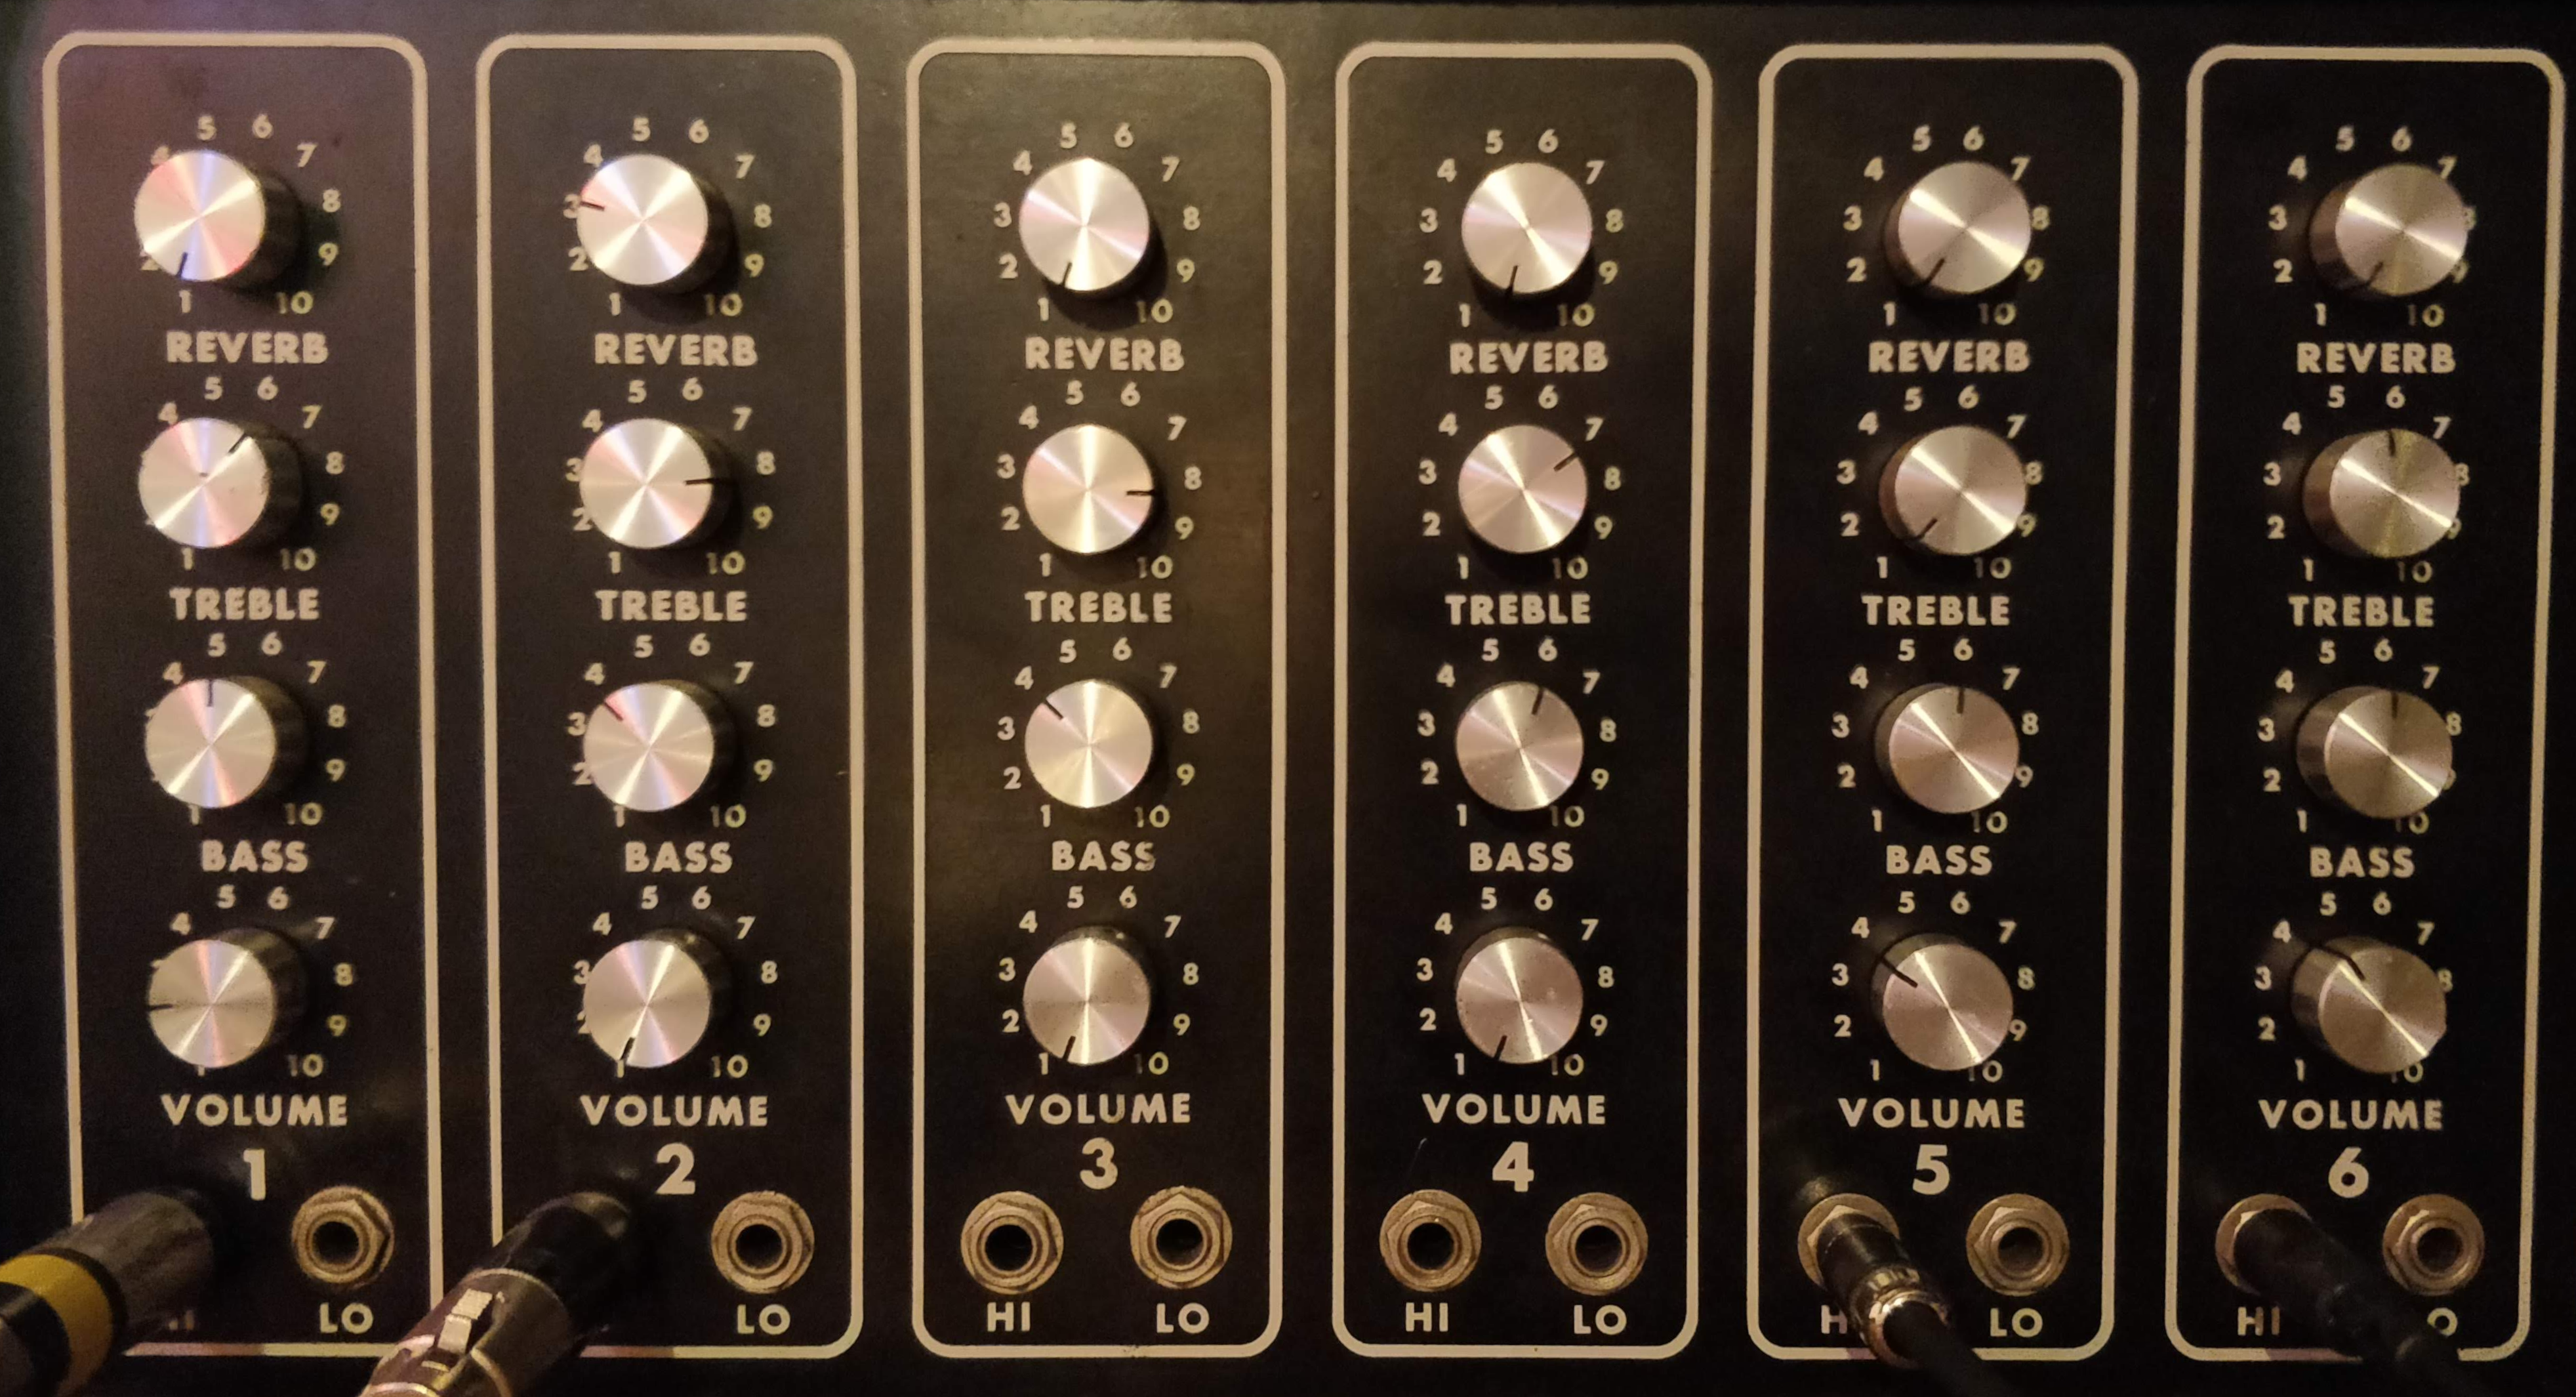
\includegraphics{amp.png}
\end{image}
One way to try and understand the machine above would be to hold all
but one of the knobs constant, and see what happens when you
``wiggle'' a single knob.  As a explicit example, let
\[
F(x,y) = x^2+2y^2
\]
Here $F$ is our ``machine'' and the variables are the ``knobs.''
Fixing $y=2$, allows us to focus our attention to all points on the
surface where the $y$-value is $2$,
\begin{image}
\begin{tikzpicture}
\begin{axis}%
[tick label style={font=\scriptsize},axis on top,
  axis lines=center,
  view={140}{30},
  name=myplot,
  %xtick=\empty,
  %ytick={5},
  %ztick={.7,-.7},
  ymin=-4.5,ymax=4.5,
  xmin=-4.5,xmax=4.5,
  zmin=-1.1, zmax=26,
  every axis x label/.style={at={(axis cs:\pgfkeysvalueof{/pgfplots/xmax},0,0)},xshift=-5pt,yshift=-1pt},
  xlabel={\scriptsize $x$},
  every axis y label/.style={at={(axis cs:0,\pgfkeysvalueof{/pgfplots/ymax},0)},xshift=4pt,yshift=-4pt},
  ylabel={\scriptsize $y$},
  every axis z label/.style={at={(axis cs:0,0,\pgfkeysvalueof{/pgfplots/zmax})},xshift=0pt,yshift=4pt},
  zlabel={\scriptsize $z$},colormap/cool
]
\addplot3[domain=-3:3,y domain=-3:3,mesh,samples y=20,very thin,z buffer=sort,  samples=25,] (x,y,{x^2+2*(y^2)});

\addplot3 [very thick,penColor, smooth,domain=-3:3,samples=20,samples y=0] ({x},{2},{x^2+8});
\end{axis}
\end{tikzpicture}
\end{image}
We can now focus our attention on the curve 
\begin{image}
\begin{tikzpicture}
\begin{axis}%
[tick label style={font=\scriptsize},axis on top,
  axis lines=center,
  view={140}{30},
  name=myplot,
  %xtick=\empty,
  %ytick={5},
  %ztick={.7,-.7},
  ymin=-4.5,ymax=4.5,
  xmin=-4.5,xmax=4.5,
  zmin=-1.1, zmax=26,
  every axis x label/.style={at={(axis cs:\pgfkeysvalueof{/pgfplots/xmax},0,0)},xshift=-5pt,yshift=-1pt},
  xlabel={\scriptsize $x$},
  every axis y label/.style={at={(axis cs:0,\pgfkeysvalueof{/pgfplots/ymax},0)},xshift=4pt,yshift=-4pt},
  ylabel={\scriptsize $y$},
  every axis z label/.style={at={(axis cs:0,0,\pgfkeysvalueof{/pgfplots/zmax})},xshift=0pt,yshift=4pt},
  zlabel={\scriptsize $z$},colormap/cool
]
\addplot3 [very thick,penColor, smooth,domain=-3:3,samples=20,samples y=0] ({x},{2},{x^2+8});
\end{axis}
\end{tikzpicture}
\end{image}
and differentiate this curve purely with respect to $x$. In a similar way, we could fix $x$ and differentiate with respect to $y$.

\begin{definition}
  Given a function $F:\R^n\to\R$, the \dfn{partial derivative} of $F$
  with respect to the $i$th variable is denoted:
  \begin{align*}
  \pp{x_i} F(x_1,x_2,\dots,x_n) &= \pp{x_i} F(\vec{x})\\
  &= \lim_{h\to 0} \frac{F(x_1,\dots,x_i+h,\dots,x_n) - F(x_1,\dots,x_n)}{h}
  \end{align*}
  This means that one should take the single-variable derivative with
  respect to $x_i$ of $F$ while treating all other variables as
  constants.
\end{definition}

\begin{onlineOnly}
  The following interactive let's you see whats going on with partial derivatives:
  \begin{center}
    \geogebra{sdfekprj}{800}{600}%https://ggbm.at/sdfekprj
  \end{center}
\end{onlineOnly}


\begin{question}
  Let $F(x,y) = x^2+2y^2$. Compute:
  \[
  \pp{x} F(x,y)
  \begin{prompt}
    = \answer{2x+0}
  \end{prompt}
  \]
  \begin{question}
    Compute
  \[
  \pp{y} F(x,y)
  \begin{prompt}
    = \answer{0+4y}
  \end{prompt}
  \]
  \end{question}
\end{question}


\begin{definition}\index{partial derivative!notation}
  There are several different notations for the partial derivative.
  We'll mainly be using these:
  \begin{align*}
    \pp{x} F(x,y,z) &= F^{(1,0,0)}(x,y,z) = F_x(x,y,z),\\
    \pp{y} F(x,y,z) &= F^{(0,1,0)}(x,y,z) = F_y(x,y,z),\\
    \pp{z} F(x,y,z) &= F^{(0,0,1)}(x,y,z) = F_z(x,y,z).
  \end{align*}
\end{definition}

\begin{question}
  Let $F(x,y) = x^2y + 2x+y^3$. Compute:
  \[
  F^{(1,0)}(x,y)
  \begin{prompt}
    = \answer{2xy+2}
  \end{prompt}
  \]
  \begin{question}
    Compute:
  \[
  F^{(0,1)}(x,y)
  \begin{prompt}
    = \answer{x^2+3y^2}
  \end{prompt}
  \]
  \end{question}
\end{question}

We have shown \textit{how} to compute a partial derivative, but it may
still not be clear what a partial derivative \textit{means}. Given
$z=F(x,y)$, $F^{(1,0)}(x,y)$ measures the rate at which $z$ changes as
only $x$ varies: $y$ is held constant. 

Imagine standing in a rolling meadow, then beginning to walk due
east. Depending on your location, you might walk up, sharply down, or
perhaps not change elevation at all. This is similar to measuring
$\pp[z]{x}$: you are moving only east (in the $x$-direction) and
not north/south at all. Going back to your original location, imagine
now walking due north (in the $y$-direction). Perhaps walking due
north does not change your elevation at all. This is analogous to
$\pp[z]{y}=0$: $z$ does not change with respect to $y$. We can see
that $\pp[z]{x}$ and $\pp[z]{y}$ do not have to be the same, or even
similar, as it is easy to imagine circumstances where walking east
means you walk downhill, though walking north makes you walk uphill.
The next example helps us visualize this.


\begin{example}
  Let $F(x,y)=-x^2-\frac{y^2}{2}+xy+10$. Find $F^{(1,0)}(2,1)$ and
  $F^{(0,1)}(2,1)$.
  \begin{explanation}
    Write with me
    \[
    \pp{x}F(x,y) = \answer[given]{-2x+y}
    \]
    and
    \[
    \pp{y}F(x,y) = \answer[given]{-y+x}
    \]
    Thus $F^{(1,0)}(2,1) = \answer[given]{-3}$ and $F^{(0,1)}(2,1) =
    \answer[given]{1}$.
  \end{explanation}
\end{example}

Whenever we do a computation in mathematics, we should ask ourselves,
``What does this mean?''
\begin{example}
   Let $F(x,y)=-x^2-\frac{y^2}{2}+xy+10$. What is the meaning of
  \begin{align*}
    F^{(1,0)}(2,1) &= -3\\
    F^{(0,1)}(2,1)&=1?
  \end{align*}
  \begin{explanation}
    First note that $F(2,1) = \answer[given]{7.5}$.  If
    $F^{(1,0)}(2,1)=-3$, this means if one ``stands'' on the surface
    at the point
    $(\answer[given]{2},\answer[given]{1},\answer[given]{7.5})$ and
    moves \wordChoice{\choice[correct]{parallel}\choice{orthogonal}}
    to the $x$-axis (so only the $x$-value changes, not the
    $y$-value), then the instantaneous rate of change in $z$ is
    $\answer[given]{-3}$. Increasing the $x$-value will
    \wordChoice{\choice{increase}\choice[correct]{decrease}} the
    $z$-value; decreasing the $x$-value will
    \wordChoice{\choice[correct]{increase}\choice{decrease}} the
    $z$-value.
    \begin{image}
      \begin{tikzpicture}
        \begin{axis}%
          [tick label style={font=\scriptsize},axis on top,
	    axis lines=center,
	    view={135}{30},
	    name=myplot,
	    %xtick=\empty,
	    %ytick={5},
	    %ztick={.7,-.7},
	    minor xtick=1,
	    minor ytick=1,
	    ymin=-.5,ymax=3.5,
	    xmin=-.5,xmax=3.5,
	    zmin=-1.1, zmax=12,
	    every axis x label/.style={at={(axis cs:\pgfkeysvalueof{/pgfplots/xmax},0,0)},xshift=-5pt,yshift=-1pt},
	    xlabel={\scriptsize $x$},
	    every axis y label/.style={at={(axis cs:0,\pgfkeysvalueof{/pgfplots/ymax},0)},xshift=4pt,yshift=-4pt},
	    ylabel={\scriptsize $y$},
	    every axis z label/.style={at={(axis cs:0,0,\pgfkeysvalueof{/pgfplots/zmax})},xshift=0pt,yshift=4pt},
	    zlabel={\scriptsize $z$},colormap/cool
	  ]
          \addplot3[domain=0:3,y domain=0:3,mesh,samples y=10,very thin,z buffer=sort,
samples=10,] (x,y,{-x^2-.5*(y^2)+x*y+10});

\addplot3 [very thick,penColor, smooth,domain=0:3,samples=20,samples y=0] ({x},{1},{-x^2+x+9.5});

\addplot3 [ultra thick,penColor2, smooth,domain=0:3.5,samples=20,samples y=0] ({x},{1},{-3*(x-2)+7.5});

\filldraw [black] (axis cs:2,1,7.5) circle (1.5pt);
\end{axis}
\end{tikzpicture}
    \end{image}
    
    If $F^{(0,1)}(2,1)=1$, this means if one ``stands'' on the surface
    at the point
    $(\answer[given]{2},\answer[given]{1},\answer[given]{7.5})$ and
    moves \wordChoice{\choice[correct]{parallel}\choice{orthogonal}}
    to the $y$-axis (so only the $y$-value changes, not the
    $x$-value), then the instantaneous rate of change in $z$ is
    $\answer[given]{1}$. Increasing the $y$-value will
    \wordChoice{\choice[correct]{increase}\choice{decrease}} the
    $z$-value; decreasing the $y$-value will
    \wordChoice{\choice{increase}\choice[correct]{decrease}} the
    $z$-value.
    \begin{image}
      \begin{tikzpicture}
\begin{axis}%
[tick label style={font=\scriptsize},axis on top,
			axis lines=center,
			view={135}{30},
			name=myplot,
			%xtick=\empty,
			%ytick={5},
			%ztick={.7,-.7},
			minor xtick=1,
			minor ytick=1,
			ymin=-.5,ymax=3.5,
			xmin=-.5,xmax=3.5,
			zmin=-1.1, zmax=12,
			every axis x label/.style={at={(axis cs:\pgfkeysvalueof{/pgfplots/xmax},0,0)},xshift=-5pt,yshift=-1pt},
				xlabel={\scriptsize $x$},
			every axis y label/.style={at={(axis cs:0,\pgfkeysvalueof{/pgfplots/ymax},0)},xshift=4pt,yshift=-4pt},
				ylabel={\scriptsize $y$},
				every axis z label/.style={at={(axis cs:0,0,\pgfkeysvalueof{/pgfplots/zmax})},xshift=0pt,yshift=4pt},
				zlabel={\scriptsize $z$},colormap/cool
			]
\addplot3[domain=0:3,y domain=0:3,mesh,samples y=10,very thin,z buffer=sort,
samples=10,] (x,y,{-x^2-.5*(y^2)+x*y+10});

\addplot3 [very thick,penColor, smooth,domain=0:3,samples=20,samples y=0] ({2},{x},{-.5*x^2+2*x+6});
\addplot3 [ultra thick,penColor2, smooth,domain=0:3.5,samples=20,samples y=0] ({2},{x},{1*(x-1)+7.5});
\filldraw [black] (axis cs:2,1,7.5) circle (1.5pt);
\end{axis}
\end{tikzpicture}
    \end{image}    
    Finally, since the magnitude of $\pp[F]{x}$ is greater than the
    magnitude of $\pp[F]{y}$ at $(2,1)$, the surface is ``steeper'' in
    the $x$-direction than in the $y$-direction.
  \end{explanation}
\end{example}

\section{Estimating partial derivatives}

Functions of several variables, especially ones that map $\R^2\to \R$
can be described by a table of values or level curves. In either case
we can estimate partial derivatives by looking at
\[
\frac{\text{change in the output}}{\text{change in the variable}}
\]
Let's do an example to make this more clear.
\begin{example}
  Let $F:\R^2\to\R$ be a differentiable function described by the
  following table of values:
  \begin{image}
    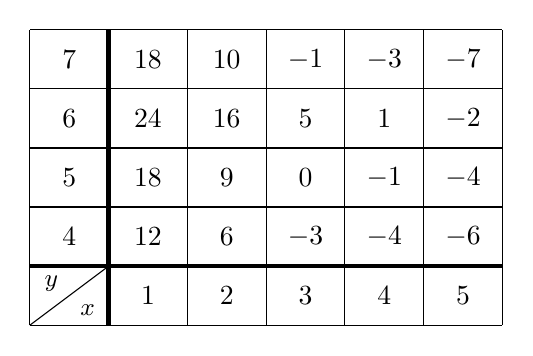
\begin{tikzpicture}[x=1cm,y=.75cm]
    \draw (0,0) grid [step=1] (6,5);
    
    \draw[ultra thick] (0,1)--(6,1);
    \draw[ultra thick] (1,0)--(1,5);
    
    \draw (0,0) -- (1,1);
    \node at (.4,.9) [below left,inner sep=1pt] {\small$y$};
    \node at (0.6,.1) [above right,inner sep=1pt] {\small$x$};
    
    %% y-values
    \node at (0.5,4.5) {$7$};
    \node at (0.5,3.5) {$6$};
    \node at (0.5,2.5) {$5$};
    \node at (0.5,1.5) {$4$};

    
    %% z-values
    %% top
    \node at (1.5,4.5) {$18$};
    \node at (2.5,4.5) {$10$};
    \node at (3.5,4.5) {$-1$};
    \node at (4.5,4.5) {$-3$};
    \node at (5.5,4.5) {$-7$};
    
    %% 
    \node at (1.5,3.5) {$24$};
    \node at (2.5,3.5) {$16$};
    \node at (3.5,3.5) {$5$};
    \node at (4.5,3.5) {$1$};
    \node at (5.5,3.5) {$-2$};
    
    %% 
    \node at (1.5,2.5) {$18$};
    \node at (2.5,2.5) {$9$};
    \node at (3.5,2.5) {$0$};
    \node at (4.5,2.5) {$-1$};
    \node at (5.5,2.5) {$-4$};
    
    %% 
    \node at (1.5,1.5) {$12$};
    \node at (2.5,1.5) {$6$};
    \node at (3.5,1.5) {$-3$};
    \node at (4.5,1.5) {$-4$};
    \node at (5.5,1.5) {$-6$};
    
    %% bottom row
    \node at (1.5,.5) {$1$};
    \node at (2.5,.5) {$2$};
    \node at (3.5,.5) {$3$};
    \node at (4.5,.5) {$4$};
    \node at (5.5,.5) {$5$};
    \end{tikzpicture}
  \end{image}
  Estimate $F^{(1,0)}(2,6)$.
  \begin{explanation}
    To estimate $F^{(1,0)}(2,6)$, we examine the change in $F(x,6)$
    between $x=1$ and $x=2$ and then between $x=2$ and $x=3$. We will
    then average these estimates to find our answer. To start look
    between $x=1$ and $x=2$:
    \begin{align*}
      \frac{F(2,6)-F(1,6)}{2-1}&= \frac{\answer[given]{16}-\answer[given]{24}}{2-1}\\
      &=\answer[given]{-8}
    \end{align*}
    Now examine the change in $F(x,6)$ between $x=2$ and $x=3$:
    \begin{align*}
      \frac{F(3,6)-F(2,6)}{3-2}&= \frac{\answer[given]{5}-\answer[given]{16}}{3-2}\\
      &=\answer[given]{-11}
    \end{align*}
    Now if we average these values together, we see:
    \[
    \eval{\pp{x} F(x,y)}_{(x,y)=(2,6)} \approx \answer[given]{-9.5}
    \]
  \end{explanation}
\end{example}

\begin{question}
  Let $F:\R^2\to\R$ be a differentiable function described by the
  following table of values:
  \begin{image}
    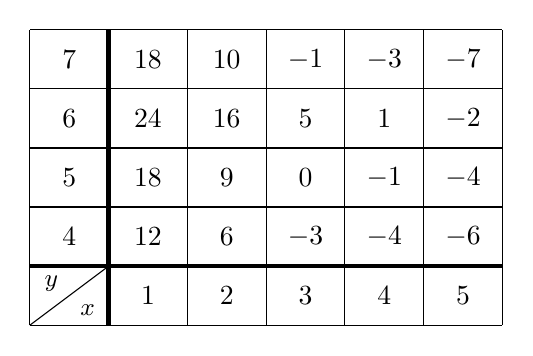
\begin{tikzpicture}[x=1cm,y=.75cm]
    \draw (0,0) grid [step=1] (6,5);
    
    \draw[ultra thick] (0,1)--(6,1);
    \draw[ultra thick] (1,0)--(1,5);
    
    \draw (0,0) -- (1,1);
    \node at (.4,.9) [below left,inner sep=1pt] {\small$y$};
    \node at (0.6,.1) [above right,inner sep=1pt] {\small$x$};
    
    %% y-values
    \node at (0.5,4.5) {$7$};
    \node at (0.5,3.5) {$6$};
    \node at (0.5,2.5) {$5$};
    \node at (0.5,1.5) {$4$};

    
    %% z-values
    %% top
    \node at (1.5,4.5) {$18$};
    \node at (2.5,4.5) {$10$};
    \node at (3.5,4.5) {$-1$};
    \node at (4.5,4.5) {$-3$};
    \node at (5.5,4.5) {$-7$};
    
    %% 
    \node at (1.5,3.5) {$24$};
    \node at (2.5,3.5) {$16$};
    \node at (3.5,3.5) {$5$};
    \node at (4.5,3.5) {$1$};
    \node at (5.5,3.5) {$-2$};
    
    %% 
    \node at (1.5,2.5) {$18$};
    \node at (2.5,2.5) {$9$};
    \node at (3.5,2.5) {$0$};
    \node at (4.5,2.5) {$-1$};
    \node at (5.5,2.5) {$-4$};
    
    %% 
    \node at (1.5,1.5) {$12$};
    \node at (2.5,1.5) {$6$};
    \node at (3.5,1.5) {$-3$};
    \node at (4.5,1.5) {$-4$};
    \node at (5.5,1.5) {$-6$};
    
    %% bottom row
    \node at (1.5,.5) {$1$};
    \node at (2.5,.5) {$2$};
    \node at (3.5,.5) {$3$};
    \node at (4.5,.5) {$4$};
    \node at (5.5,.5) {$5$};
    \end{tikzpicture}
  \end{image}
  Estimate $F^{(0,1)}(2,6)$.
  \begin{prompt}
    \[
    F^{(0,1)}(2,6)\approx \answer{.5}
    \]
  \end{prompt}
  \begin{hint}
    Work as we did in the example above, finding two estimates and taking their averages. 
  \end{hint}
\end{question}

We can also estimate partial derivatives by looking at level curves.

\begin{example}
  Let $F:\R^2\to\R$ be described by the level curves below:
    \begin{image}
      \begin{tikzpicture}
        \begin{axis}%
          [tick label style={font=\scriptsize},axis on top,
	    axis lines=center,
	    %view={30}{30},
	    %name=myplot,
            %width=5in,
	    xtick={0,1,...,6},
            ytick={0,1,...,5},
	    %ytick={5},
	    %ztick={.7,-.7},
	    ymin=-.2,ymax=5,
	    xmin=-.2,xmax=6,
            grid=major,%width=3in,height=3in,
            grid style={dashed, gridColor},
	    every axis x label/.style={at={(axis cs:\pgfkeysvalueof{/pgfplots/xmax},0,0)},xshift=5pt,yshift=0pt},
	    xlabel={\scriptsize $x$},
	    every axis y label/.style={at={(axis cs:0,\pgfkeysvalueof{/pgfplots/ymax},0)},xshift=4pt,yshift=2pt},
	    ylabel={\scriptsize $y$},
	  ]
          \addplot[very thick, penColor,smooth] coordinates{
            (0,0) (4,1) (5,2) (6,2.5)
          };

          \addplot[very thick, penColor,smooth] coordinates{
            (0,1) (4,2) (6,3)
          };

          \addplot[very thick, penColor,smooth] coordinates{
            (0,1.5) (1,2) (4,4) (6,5)
            };

          \node[penColor,fill=white] at (axis cs:2,.5) {$17$};
          \node[penColor,fill=white] at (axis cs:2,1.5) {$13$};
          \node[penColor,fill=white] at (axis cs:2,2.66) {$7$};

          \addplot[color=black,fill=black,only marks,mark=*] coordinates{(4,2)};  %% closed hole          
        \end{axis}
      \end{tikzpicture}
    \end{image}
    The height of the level curve is marked on the curve, and we are
    given a point $(4,2)$.  Estimate $F^{(1,0)}(4,2)$.   
  \begin{explanation}
    To estimate $F^{(1,0)}(4,2)$ we examine the change between the
    level curve that $\vec{p}$ is on, and the nearest level curve
    found by traveling on a line parallel to the $x$-axis. Starting at
    $\vec{p}$ and moving to the left on a line parallel to the
    $x$-axis, we see
    \begin{align*}
      \frac{F(4,2)-F(1,2)}{4-1}&= \frac{\answer[given]{13}-\answer[given]{7}}{4-1}\\
      &=\answer[given]{2}
    \end{align*}
    We also should examine the change between the closest level curve
    when moving to the right:
    \begin{align*}
      \frac{F(5,2)-F(4,2)}{5-4}&= \frac{\answer[given]{17}-\answer[given]{13}}{5-4}\\
      &=\answer[given]{4}
    \end{align*}
    Now if we average these values together, we see:
    \[
    \eval{\pp{x} F(x,y)}_{(x,y)=(2,6)} \approx \answer[given]{3}
    \]
  \end{explanation}
\end{example}



\begin{question}
  Let $F:\R^2\to\R$ be described by the level curves below:
    \begin{image}
      \begin{tikzpicture}
        \begin{axis}%
          [tick label style={font=\scriptsize},axis on top,
	    axis lines=center,
	    %view={30}{30},
	    %name=myplot,
            %width=5in,
	    xtick={0,1,...,6},
            ytick={0,1,...,5},
	    %ytick={5},
	    %ztick={.7,-.7},
	    ymin=-.2,ymax=5,
	    xmin=-.2,xmax=6,
            grid=major,%width=3in,height=3in,
            grid style={dashed, gridColor},
	    every axis x label/.style={at={(axis cs:\pgfkeysvalueof{/pgfplots/xmax},0,0)},xshift=5pt,yshift=0pt},
	    xlabel={\scriptsize $x$},
	    every axis y label/.style={at={(axis cs:0,\pgfkeysvalueof{/pgfplots/ymax},0)},xshift=4pt,yshift=2pt},
	    ylabel={\scriptsize $y$},
	  ]
          \addplot[very thick, penColor,smooth] coordinates{
            (0,0) (4,1) (5,2) (6,2.5)
          };

          \addplot[very thick, penColor,smooth] coordinates{
            (0,1) (4,2) (6,3)
          };

          \addplot[very thick, penColor,smooth] coordinates{
            (0,1.5) (1,2) (4,4) (6,5)
            };

          \node[penColor,fill=white] at (axis cs:2,.5) {$17$};
          \node[penColor,fill=white] at (axis cs:2,1.5) {$13$};
          \node[penColor,fill=white] at (axis cs:2,2.66) {$7$};

          \addplot[color=black,fill=black,only marks,mark=*] coordinates{(4,2)};  %% closed hole          
        \end{axis}
      \end{tikzpicture}
    \end{image}
    The height of the level curve is marked on the curve, and we are
    given a point $(4,2)$.  Estimate $F^{(0,1)}(4,2)$.
  \[
  \begin{prompt}
      F^{(0,1)}(4,2)\approx \answer{-3.5}
  \end{prompt}
  \]
  \begin{hint}
    Work as we did in the example above, finding two estimates and taking their averages. 
  \end{hint}
\end{question}


\section{Combining partial derivatives}

While a function $f:\R\to\R$ only has one second derivative. However,
functions $F:\R^2\to \R$ have $4$ \textit{second partial derivatives}
and functions $F:\R^3\to\R$ have $9$ \textit{second partial
  derivatives}! Don't run off yet, things get better.

\begin{definition}
  Let $F:\R^n\to\R$ be continuous on an open set $S$.
  \begin{itemize}\index{partial derivative!pure}
  \item The \dfn{second pure partial derivative} of $F$ with respect to $x$ then $x$ is
    \[
    \pp{x}\left(\pp[F]{x}\right) = F_{xx}=\frac{\partial^2 F}{\partial x^2} = \left(F^{(1,0)}\right)^{(1,0)}= F^{(2,0)}
    \]
  \item The \dfn{second pure partial derivative} of $F$ with respect to
    $y$ then $y$ is
    \[
    \pp{y}\left(\pp[F]{y}\right) = F_{yy}=\frac{\partial^2F}{\partial y^2} = \left(F^{(0,1)}\right)^{(0,1)} = F^{(0,2)}
    \]
\end{itemize}
Moreover, there is also the notion of
a \dfn{mixed partial derivative},
\[
\frac{\partial}{\partial y}\left(\frac{\partial F}{\partial x}\right) = \frac{\partial^2F}{\partial y\partial x} = \left(F_x\right)_y = F_{xy}
\]
and
\[
\frac{\partial}{\partial x}\left(\frac{\partial F}{\partial y}\right) = \frac{\partial^2F}{\partial x\partial y} = \left(F_y\right)_x =F_{yx}
\]
The notation $F^{(1,1)}$ is ambiguous, it does not state which
derivative should be taken first. As we will see, in practice this is
not too much of a problem.
\index{partial derivative!mixed}\index{partial derivative!second derivative}\index{derivative!mixed partial}
\end{definition}


\begin{question}
  Consider:
  \[
  F(x,y) = x^3y^2 + 2xy^3+\cos(x)
  \]
  Find six first and second partial derivatives.
  \begin{prompt}
    \begin{align*}
      \pp[F]{x} &= \answer{3x^2y^2+2y^3-\sin(x)}\\
      \pp[F]{y} &= \answer{2x^3y+6xy^2}\\
      \frac{\partial^2F}{\partial x^2} &= \answer{6xy^2-\cos(x)}\\
      \frac{\partial^2F}{\partial y^2} &= \answer{2x^3+12xy}\\
      \frac{\partial^2F}{\partial y\partial x} &= \answer{6x^2y+6y^2}\\
      \frac{\partial^2F}{\partial x\partial y} &= \answer{6x^2y+6y^2}
    \end{align*}
  \end{prompt}
\end{question}
Notice how above $\frac{\partial^2F}{\partial y\partial
  x}=\frac{\partial^2F}{\partial x\partial y}$. The next theorem states
that it is not a coincidence.

\begin{theorem}[Mixed Partial Derivatives]
  Let $F:\R^2\to \R$ be a function where
  \[
  \frac{\partial^2F}{\partial y\partial x}\quad\text{and}\quad\frac{\partial^2F}{\partial x\partial y}
  \]
  are continuous on an open set $S$. Then for each point $(x,y)$ in
  $S$, $\frac{\partial^2F}{\partial y\partial
    x}=\frac{\partial^2F}{\partial x\partial y}$.
  A similar result is true for functions $F:\R^n\to \R$.
\end{theorem}

Finding $\frac{\partial^2F}{\partial y\partial x}$ and
$\frac{\partial^2F}{\partial x\partial y}$ independently and comparing
the results provides a convenient way of checking our work.


\section{The gradient vector}\index{gradient}


Given a function $F:\R^n\to\R$, we often want to work with all of
first partial derivatives simultaneously. In this case, we will work with the vector:
\[
\vector{\pp[F]{x_1},\pp[F]{x_2},\dots,\pp[F]{x_n}}
\]
As we will see, for functions of several variables, this vector will
play the role that the derivative did for functions of a single variable. This vector is called the \textit{gradient vector}.

\begin{definition}
  Let $F:\R^n\to \R$ be a function whose first partial derivatives
  exist, the \dfn{gradient}
  \[
  \grad F = \vector{\pp[F]{x_1},\pp[F]{x_2},\dots,\pp[F]{x_n}}
  \]
  is a vector-valued function of $n$ variables. 
\end{definition}

The upside-down triangle in the notation for the gradient sometimes
called a \textit{del}. It is also known as a \textit{nabla}. You can
think of the $\grad$ as the vector:
\[
\grad = \vector{\pp{x_1},\pp{x_2},\dots,\pp{x_n}}
\]
and hence when one writes: $\grad F$, you are literally distributing
the $F$ across the vector, just as a scalar acts on a vector.


\begin{remark}
The gradient is defined at points in the domain where the partial
derivatives are defined. The gradient of a function of two variables
lives in $\R^2$. The gradient of a function of three variables lives
in $\R^3$. Generally the gradient of a function of $n$ variables lives
in $\R^n$.
\begin{onlineOnly}
  We can see this in the interactive below. 
  \begin{center}
    \geogebra{wd5mrudh}{800}{600} %https://ggbm.at/wd5mrudh
  \end{center}
  The gradient at each point is a vector pointing in the $(x,y)$-plane.
\end{onlineOnly}


\end{remark}




Try your hand at some casual computations.

\begin{question}
  Let $F(x,y) = \sin(x)\cos(y)$, compute:
  \[
  \grad F(x,y)
  \begin{prompt}
    = \vector{\answer{\cos(x)\cos(y)},\answer{-\sin(x)\sin(y)}}
  \end{prompt}
  \]
  \begin{question}
Above, note that $\grad F(x,y)$ is a vector whose components are
functions of $x$ and $y$, hence it is a vector-valued function.  We
can evaluate functions at actual points in their domain.  For
instance, if $\vec{p}= \vector{\pi/3,\pi/3}$ we compute:
    \[
    \grad F(\vec{p})
    \begin{prompt}
      =\vector{\answer{1/4},\answer{-3/4}}.
    \end{prompt}
    \]
  \end{question}
\end{question}

And now in three variables.

\begin{question}
  Let $F(x,y,z) = ze^{-7xy}$, compute:
  \[
  \grad F(x,y,z)
  \begin{prompt}
    = \vector{\answer{z e^{-7xy}(-7)y},\answer{z e^{-7xy}(-7)x}, \answer{e^{-7xy}}}
  \end{prompt}
  \]
  \begin{question}
    Let $\vec{p}= \vector{1,0,1/7}$. Compute:
    \[
    \grad F(\vec{p})
    \begin{prompt}
      =\vector{\answer{0},\answer{-1},\answer{1}}
    \end{prompt}
    \]
  \end{question}
\end{question}


This is just your first taste of the gradient vector. Much more will be coming soon. 



\end{document}
